%; whizzy chapter
% -initex iniptex -latex platex -format platex -bibtex jbibtex -fmt fmt
% 以上 whizzytex を使用する場合の設定。

%     Kansai Debian Meeting resources
%     Copyright (C) 2007 Takaya Yamashita
%     Thank you for Tokyo Debian Meeting resources

%     This program is free software; you can redistribute it and/or modify
%     it under the terms of the GNU General Public License as published by
%     the Free Software Foundation; either version 2 of the License, or
%     (at your option) any later version.

%     This program is distributed in the hope that it will be useful,
%     but WITHOUT ANY WARRANTY; without even the implied warranty of
%     MERCHANTABILITY or FITNESS FOR A PARTICULAR PURPOSE.  See the
%     GNU General Public License for more details.

%     You should have received a copy of the GNU General Public License
%     along with this program; if not, write to the Free Software
%     Foundation, Inc., 51 Franklin St, Fifth Floor, Boston, MA  02110-1301 USA

%  preview (shell-command (concat "evince " (replace-regexp-in-string "tex$" "pdf"(buffer-file-name)) "&"))
% 画像ファイルを処理するためにはebbを利用してboundingboxを作成。
%(shell-command "cd image200708; ebb *.png")

%%ここからヘッダ開始。

\documentclass[mingoth,a4paper]{jsarticle}
\usepackage{kansaimonthlyreport}
\usepackage[dvipdfmx]{xy}
\usepackage{etex}
\usepackage{ulem}

% 日付を定義する、毎月変わります。
\newcommand{\debmtgyear}{2014}
\newcommand{\debmtgdate}{22}
\newcommand{\debmtgmonth}{6}
\newcommand{\debmtgnumber}{85}

\def\fixme#1{{\color{red}{#1}}}

\begin{document}

\begin{titlepage}

% 毎月変更する部分、本文の末尾も修正することをわすれずに

 第\debmtgnumber{}回 関西 Debian 勉強会資料

\vspace{2cm}

\begin{center}
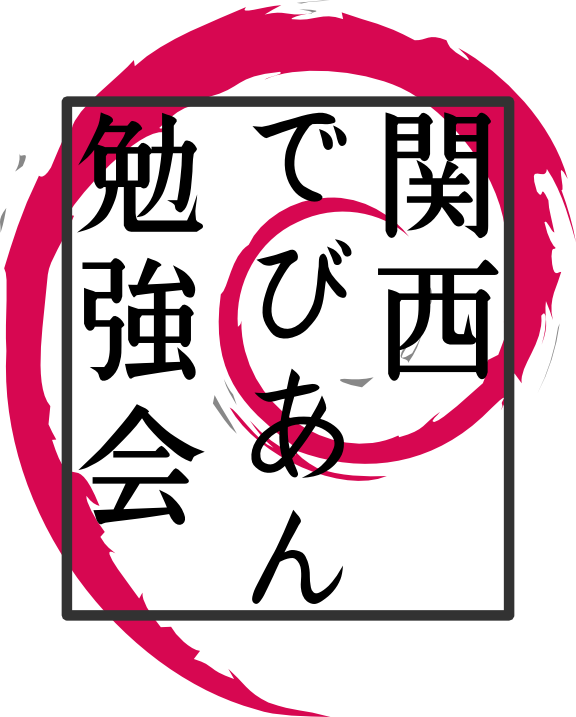
\includegraphics{image200802/kansaidebianlogo.png}
\end{center}

\begin{flushright}
\hfill{}関西 Debian 勉強会担当者 佐々木・倉敷・のがた・かわだ・八津尾 \\
\hfill{}\debmtgyear{}年\debmtgmonth{}月\debmtgdate{}日
\end{flushright}

\thispagestyle{empty}
\end{titlepage}

\dancersection{Introduction}{Debian JP}

\vspace{1em}

 関西Debian勉強会はDebian GNU/Linuxのさまざまなトピック
 (新しいパッケージ、Debian特有の機能の仕組、Debian界隈で起こった出来事、
 などなど)について話し合う会です。

 目的として次の三つを考えています。
 \begin{itemize}
  \item MLや掲示板ではなく、直接顔を合わせる事での情報交換の促進
  \item 定期的に集まれる場所
  \item 資料の作成
 \end{itemize}

 それでは、楽しい一時をお過ごしください。

\newpage

\begin{minipage}[b]{0.2\hsize}
 {\rotatebox{90}{\fontsize{80}{80}
{\gt 関西 Debian 勉強会}}}
\end{minipage}
\begin{minipage}[b]{0.8\hsize}
\hrule
\vspace{2mm}
\hrule
\setcounter{tocdepth}{1}
\tableofcontents
\vspace{2mm}
\hrule
\end{minipage}

\dancersection{最近のDebian関係のイベント報告}{Debian JP}

\subsection{第84回関西Debian勉強会}

84回目の関西Debian勉強会は5月25日(日)に、福島区民センターで行なわれまし
た。

もくもくの会中心の開催でしたが、キーサイン、systemdの話しが話題にあがり
ました。今回はその続きという感じでsystemdのお話しになります。

\subsection{第114回東京エリアDebian勉強会}

114回目の東京エリアDebian勉強会は6月14日(土)に株式会社スクウェア・エニッ
クス 会議室で行なわれました。

吉田さんによる「GPG 秘密鍵取り扱い方法の提案」ともくもくの会の形式で行
なわれました。

みなさん悩みどころのGPG秘密鍵の扱いをどうするかについて、このセッショ
ンではGPG秘密鍵をRAID5のように複数のファイルとパリティに分割して管理す
るアイデアが紹介されています。面白い方法だと思いますのでぜひ資料に目を
通してみてください。

\subsection{Debian Project}

\subsubsection{MATE 1.8}
MATE Packaging Teamより「MATE 1.8 has now fully arrived in Debian」
\footnote{\url{https://lists.debian.org/debian-devel/2014/06/msg00041.html}}
とMATE 1.8がDebianに追加されたよとアナウンスがありました。
MATEはGNOME2からフォークしたデスクトップ環境プロジェクトです。GNOME3を
好ましいと思っていない方にとっては好評で、よほどうれしかったのか10分も
経たないうちにNorbert Preiningさんから
\begin{quote}
  *big*big*big* thanks for all your work, it is very very much appreciated!
\end{quote}
と感謝のメールが飛んでいました。

すでに、unstableだけでなくtesting、wheezy-backportsにもパッケージが用意
されていますので試してみたい方は次のメタパッケージをインストールしてみ
てください。
\begin{commandline}
  $ sudo apt-get install mate-desktop-environment
\end{commandline}
%$

\subsubsection{Debian 6 ``squeeze'' LTS}
Debian Projectから「Debian 6 debuts its long term support period」
\footnote{\url{https://lists.debian.org/debian-announce/2014/msg00004.html}}
とDebian初となるLTS (Long Term Support)をDebian GNU/Linux 6.0 ``squeeze''
に提供しますとアナウンスがありました。このサポートは2016年2月まで続け
られる予定です。

LTSを利用してみようと思われる方は「How to use the updates from LTS」
\footnote{\url{lhttps://wiki.debian.org/LTS/Using}}
によく目を通してから利用してください。全アーキテクチャ、全パッケージが
LTSサポートの対象ではありませんので十分に注意してください。
どのパッケージがLTSのサポートの対象外となるかはdebian-security-support
パッケージを使って確認することができます。

\subsubsection{Berkeley DB}
「New project goal: Get rid of Berkeley DB (post jessie)」
\footnote{\url{https://lists.debian.org/debian-devel/2014/06/msg00328.html}}
でBerkeley DBは死んだのでLMDBのような別の実装に置き換えようという提案
がありました。
ちょうど一年ほど前に「Berkeley DB 6.0 license change to AGPLv3」
\footnote{\url{https://lists.debian.org/debian-devel/2013/07/msg00031.html}}
で話題になったAGPLv3へのライセンス変更によるものです。このため未だ
Berkeley DB 6.0はDebianのリポジトリに入っていません。
\footnote{バージョン6.0.19がexperimentalに入ったことがあるのですが、そ
の後5.3.21に戻されました。}

先月もGhostscriptがAGPLにリライセンスされた話題がありましたが、ライセ
ンス変更の問題は悩ましいです。

\dancersection{事前課題}{Debian JP}

今回の課題は以下の通りです。
\begin{screen}
  \begin{enumerate}

  \item %
    もくもくの会で行なう作業、質問などの課題を用意して教えてください。
    (電源とネットワーク(WiMAXなど)はありますが、それ以外の作業に必要な
    環境はご用意ください。)

  \item %
    前回(第84回)の勉強会に参加された方は、前回の作業や課題がその後どう
    なったか結果を教えてください。

  \item %
    LT(ライトニングトーク) 歓迎です。何かお話したい方はタイトルを下さい。

  \item %
    DebianでInitとしてsystemdが動作する環境を用意してきて下さい。
    仮想環境でかまいません。unstableをお使いの方はsystemd-sysvパッケー
    ジを導入するとsysvinit-coreがreplaceされてInitとしてsystemdが動作
    するようになります。

  \end{enumerate}
\end{screen}

参加者の皆さんの解答は以下の通りです:

\begin{prework}{ かわだてつたろう }
  \begin{enumerate}
  \item uim-skkを使用しているのですが、
    \begin{itemize}
    \item chromiumでtitanpadにかな入力できない
    \item xmonad+gnucacheでかな入力できない
    \end{itemize}
    のをなんとかしたい
  \end{enumerate}
\end{prework}

\begin{prework}{ 佐々木洋平 }
  申し込みわすれてたわー。

  \begin{enumerate}
  \item jekyll の依存が newqueue から unstable に落ちたので、ようやく
    new upstream を upload できます。
  \end{enumerate}

\end{prework}

\begin{prework}{ 木下 }
  \begin{enumerate}
  \item
    \begin{enumerate}
    \item Eucalyptus(プライベートクラウドとして)の調査・研究
    \item グリッドコンピューティング関連の調査・研究
      \begin{itemize}
      \item GlobusToolkitで何ができる?

        →AndroidOSのクロスコンパイルで使えたら嬉しいかも。
      \end{itemize}
    \item Debian7 on PANDABOARDの調査・研究
      \begin{itemize}
      \item WiFiモジュール(On Board:TI製)の有効化
      \item GPUデバイスドライバの有効化
      \end{itemize}
    \end{enumerate}
  \item ※前回(第84回)は欠席だった為、第83回の内容になります。
    \begin{enumerate}
    \item Eucalyptus(プライベートクラウドとして)の調査・研究

      実績:インスタンスの保存と自動化に成功
      \begin{itemize}
      \item 保存したインスタンスを起動させるとネットワーク接続が絶たれてしまっていた原因

        →ファイル:/etc/udev/rules.d/70-persistent-net.rulesにNICデバイス情報が残っていると
        新たにNICデバイス情報が登録されてしまい、NIC番号が変更され、通信不可となっていた。

        ※Eucalyptus関係者の方のお話では、「Debian用ツールのバグかも」とのこと。
        インスタンス保存にクリアすることで解決した。
      \item インスタンスをOSイメージファイル化し、ハイパーバイザ上にバックアップする

        スクリプトを作成し、crontabで定期的に起動できるようになった。
      \end{itemize}
    \item DistCCの調査・研究

      実績:上記プライベートクラウドシステムを用いて複数のVMで分散コンパイルさせる
      環境構築に成功。
      \begin{itemize}
      \item ビルドマシン(distccクライアント)とVM(distccサーバ)4台で
        PANDABOARD(OS:Android4.0.4)用FWを分散コンパイルさせ、
        コンパイル時間の短縮が可能となった。
      \end{itemize}
      課題:AndroidOSの場合、JAVAのコンパイル箇所がかなり存在するので、
      この部分が複数マシンで分散コンパイルできるようになれば、
      かなりのコンパイル時間の短縮となりそうなので、このあたりについて再調査必要。
    \item グリッドコンピューティング関連の調査・研究

      実績:保留
    \item Debian7 on PANDABOARDの調査・研究

      実績:保留
    \end{enumerate}
  \end{enumerate}
\end{prework}

\begin{prework}{ takata }
  \begin{enumerate}
  \item 課題:LUKSパーティションのパスワード入力を省略する件(未解決)

    keyfileを登録してみましたが、依然として swapパーティションに関して
    は起動時にパスワードを聞かれます。ググってみると同様の問題がいくつ
    かヒットするようなので、もくもくの会の時間でもう少し調べてみたいと
    思っています。

    stop crypttab asking for password for swap

    \url{http://askubuntu.com/questions/43432/stop-crypttab-asking-for-password-for-swap}

    ちなみに、"/"パーティションの keyfileでトラブりました。
    間違えて追加しすぎてしまった key\_{}slotを cryptsetup luksRemoveKey
    で削除しようとしたのですが、パスワードを登録した key\_{}slotを誤っ
    て削除してしまい、cryptsetup luksAddKeyでキーを登録できなくなるばか
    りかパスワードが解除できなくなってしまい(No key available with this passphrase.)、
    一瞬冷や汗が出ました。幸い、keyfileを設定した Key Slotが残っていたので、
    cryptsetup luksAddKey --key-file=...で回避でき何とか事なきを得ましたが、
    Key Slotを削除する場合はくれぐれもご注意ください。

  \item インターネットからの22番ポート(ssh)への不正アクセスについて

    教えていただいたとおり、fail2banを適用することで不正アクセスに対し
    て有効にブロックできているようです。ありがとうございました。
  \end{enumerate}
\end{prework}

\clearpage

\begin{prework}{ 西山和広 }
  \begin{enumerate}
  \item ansible でのサーバー設定を進めたいです。
  \item 前回不参加です。
  \item blog の記事から \verb+^+Xg の話を予定しています。
  \item 用意しておきます。
  \end{enumerate}
\end{prework}

\begin{prework}{ yyatsuo }
  \begin{enumerate}
  \item kernel-handbook の日本語訳をそろそろなんとかします
    あとは某雑誌の記事査読とか
  \item fcitx-skk new que に入りました!
    (new que で止まってるとも言います)
  \item 仕事の愚痴なら溜まってますよ?
  \item もう入ってる
  \end{enumerate}
\end{prework}

\begin{prework}{ 榎真治 }

  Debian wheezyでAnthyを使っていますが、日本語入力の変換効率(候補が期
  待したような順番で並んでくれないなど)がいまひとつと感じていますので、
  環境を変更してみたいと考えています。

  お勧めの方法はありますか?

  mozcを試すとしたらuim,ibusなどのどれがお勧めですか?
\end{prework}

\begin{prework}{ 坂本 貴史 }
  \begin{enumerate}
  \item 英語ドキュメントをTexフォーマットで作成しているので、その続きを書きます。
  \item 前回は参加していません
  \item 「Linuxのドライバメンテナになった体験記」というタイトルで短いセッションをする予定です
  \end{enumerate}
\end{prework}

\begin{prework}{ lurdan }
  \begin{enumerate}
  \item 手持ちパッケージの bug squash
  \item webwml-git は CI できるようにはなったけど、運用が煩雑なので再検討中です
  \end{enumerate}
\end{prework}

\begin{prework}{ 川江 }
  \begin{enumerate}
  \item emacsにて、HTML5形式のサイトの作成。で、wed-mode.elがdebianの
    パッケージにないのですが、これって「anthy-el」のようにパッケージに
    できます? というか「.el」ファイルというのはそもそも何?
  \end{enumerate}
\end{prework}

\begin{prework}{ Hiroyuki Nagata }
  \begin{enumerate}
  \item RFSのやり方、GPG鍵の交換 … 今度はある程度準備をしてくるつもり
  \item GPG鍵を作成しました、Mac Book ProにDebian jessieをインストールしました
  \item 今月はむりかもしれませんがDebianでルータ構築とか
  \end{enumerate}
\end{prework}

\dancersection{Debian での systemd とのつきあい方}{佐々木 洋平}

\begin{quote}
  Yes, it is written systemd, not system D or System D, or even
  SystemD. And it isn't system d either. \\
  \begin{flushright}
    Spelling - \texttt{http://www.freedesktop.org/wiki/Software/systemd/}
  \end{flushright}
\end{quote}

\subsection{はじめに}

少し前の話ですが、次期Debian安定版JessieでのデフォルトのInitとしてsystemdが採用されました。
勉強会参加者の皆様におかれましては、% 「最近Debian関連のイベント報告」で紹介(?)された、
\texttt{debian-devel@lists.debian.org}へ流れた\sout{品の無い}悲鳴(?)も記憶に新しいことでしょう
\footnote{%
Fsck SystemD and its developers and its users. GR to override this please.\\
 \href{https://lists.debian.org/debian-devel/2014/02/msg00316.html}{\texttt{https://lists.debian.org/debian-devel/2014/02/msg00316.html}}%
}。

色々な意見はあるでしょうけれども、
「デフォルト」として採用される以上(好むと好まざるとにかかわらず)Debianの開発者(含ワナビー)にとってsystemdの知識は必須事項になりそうです。
そんな訳で、systemdそのものについて調べた結果とDebianにおける現状についてまとめてみます。%
ちなみに主にテストした環境は以下の通り:
\begin{commandline}
% LANG=C date
Sat Jun 21 10:15:59 JST 2014
% lsb_release -a
No LSB modules are available.
Distributor ID: Debian
Description:    Debian GNU/Linux unstable (sid)
Release:        unstable
Codename:       sid
% dpkg -l | grep systemd
ii  libpam-systemd:amd64        204-10   amd64   system and service manager - PAM module
ii  libsystemd-daemon0:amd64    204-10   amd64   systemd utility library
ii  libsystemd-id128-0:amd64    204-10   amd64   systemd 128 bit ID utility library
ii  libsystemd-journal0:amd64   204-10   amd64   systemd journal utility library
ii  libsystemd-login0:amd64     204-10   amd64   systemd login utility library
ii  systemd                     204-10   amd64   system and service manager
ii  systemd-gui                 1:3-2    all     transitional package for systemd-ui
ii  systemd-sysv                204-10   amd64   system and service manager - SysV links
ii  systemd-ui                  3-2      amd64   graphical frontend for systemd
\end{commandline}
\noindent
本原稿の執筆時間がよくわかります\footnote{%
  lsb-baseとlsb-releaseしかインストールしていないので%
  \texttt{lsb\_release -a}の出力結果はこんなモンです。
}。
%
一応whezzy + wheezy-backportsでもテストはしてみましたが。

...しかし, v204 って...。

\subsection{そもそも systemd ってナニよ?}

systemdはLennart Poettering氏%
\footnote{Red Hat Inc.のエンジニアさんです。%
  systemdの開発者だけでなく様々なフリーソフトウェアの開発者でもあります。%
  例えばPulseAudioとかAvahiなんかのメイン開発者でもありますね。}%
によって開発されているInitの代替プログラムで\sout{す}した。
今では単なる「Initの代替」というより「Linuxのサービス(デーモン)管理フレームワーク」となっています。
開発は
\texttt{freedesktop.org}\footnote{%
  \href{http://www.freedesktop.org/wiki/Software/systemd/}{\texttt{http://www.freedesktop.org/wiki/Software/systemd/}}%
}で行なわれており、ライセンスはLGPL-2.1+、最新バージョンはv214となっています。

「Linuxのサービス(デーモン)管理フレームワーク」としてのsystemdの特徴は
\begin{enumerate}[topsep=1zw]
\item Initとして、SysVおよびLSB init script との互換性の提供。
\item サービスの起動をソケットとバス(D-Bus)で行なう。
\item サービス間の依存関係を明確にし、よりアグレッシブに並列起動する。
\item オンデマンドなサービスの起動。
\item プロセス管理をpidではなくcgroups(control groups)で行なう。
\end{enumerate}
といった所です。

既にLinuxカーネル用のデバイス管理ツールであるudevがsystemdのソースにマージされており、
デバイスの状態に応じてオンデマンドにサービスが起動したりします。
将来的にはcronやacpidの代替機能も提供する予定らしいです\footnote{%
  ここまで来るとやりすぎな感も否めませんが...。
}。
その他、systemdに関する開発者の思想、現状に関しては
\begin{itemize}
\item %
  \href{http://0pointer.de/blog/projects/systemd.html}{\texttt{http://0pointer.de/blog/projects/systemd.html}}
\item %
  \href{http://0pointer.de/blog/projects/systemd-for-admins-1.html}{\texttt{http://0pointer.de/blog/projects/systemd-for-admins-1.html}}
  から始まる一連のエントリ\footnote{現在\#20まであります。長くて読むの辛い...。}
\end{itemize}
が非常に参考になるでしょう。

\subsection{Debian で使うには?}

systemdの必要要件は以下の通りです:
\begin{enumerate}[topsep=1zw]
\item Linuxカーネルのバージョンは2.6.39以上
\item 以下の機能が有効となっていること
  \begin{itemize}[topsep=0zw]
  \item devtmpfs
  \item fanotify
  \item autofs4
  \item cgroups
  \end{itemize}
\end{enumerate}
カスタムカーネルを使用されている場合には、カーネルのバージョン等にご注意下さい。

Debianでパッケージとして提供されているsystemdのバージョンは
\begin{itemize}[topsep=1zw]
\item wheezy: v44
\item wheezy-backports: 204-8\~{}bpo70+1
\item jessie/sid: 204-10
\end{itemize}
です。以下、パッケージとして提供されている最新版であるv204のお話をします\footnote{%
  ちなみに、v44を使用する場合の手順は、
  \texttt{systemd} を install →
  起動時に \texttt{init=/lib/systemd/systemd}と指定する or grub エントリの書き換えを行なう、です。
}
では導入してみましょう。wheezyをお使いの方はwheezy-backportsを有効にして下さい。
initをsysvinitから置き換えるために、\texttt{systemd-sysv}を導入します。
\begin{commandline}
% sudo aptitude install systemd-sysv -t wheezy-backports <-- wheezy の場合
% sudp aptitude install systemd-sysv                     <-- jessie/sid の場合
\end{commandline}
wheezyの場合にはsysvinitがcoreパッケージなので、インストール時の依存関係解決に多少手間どるかもしれません。
以下のパッケージが依存関係でインストールされます。
\begin{commandline}
===============================================================================
[インストール] libpam-systemd:amd64
[インストール] libsystemd-journal0:amd64
[インストール] libudev1:amd64
[インストール] systemd:amd64
[インストール] systemd-sysv:amd64
[削除] sysvinit:amd64
[更新] libsystemd-daemon0:amd64 44-11+deb7u4 -> 204-8~bpo70+1
[更新] libsystemd-login0:amd64 44-11+deb7u4 -> 204-8~bpo70+1
===============================================================================
\end{commandline}
インストールが終わったら reboot します。...無事起動できたでしょうか?

systemdはbootプロセスの解析ツールがあり、起動時にかかった時間が直ぐにわかります。
\begin{commandline}
% systemd-analyze
Startup finished in 1.632s (kernel) + 3min 2.710s (userspace) = 3min 4.343s
\end{commandline}
...あれ?
\begin{commandline}
% systemd-analyze blame
       3min 12ms dnsmasq.service
        2.074s systemd-udev-settle.service
         630ms psd.service
         307ms NetworkManager.service
         127ms squid3.service
         106ms bluetooth.service
          98ms udisks2.service
          96ms exim4.service
          93ms keyboard-setup.service
          87ms bootlogs.service
          87ms avahi-daemon.service
          80ms resolvconf.service
          76ms console-setup.service
          74ms networking.service
          73ms systemd-logind.service
          69ms netfilter-persistent.service
          64ms console-kit-log-system-start.service
          ...以下略...
\end{commandline}
燦然と輝く\textbf{3min 12ms dnsmasq.service}。…おかしい。これはおかしい。

\subsection{現状どうなのよ?}

気を取りなおして。

\subsubsection{systemdの用語}
systemdを理解するために、先ずは用語を確認しましょう。
\begin{itemize}
\item ユニット(unit): \\
  SysVinitの初期化スクリプトにまとめて含まれていた個々の処理を抜き出した最小単位。
  個々のUnitはそれぞれ以下の通り:
  \begin{itemize}
  \item サービス(\texttt{.service}): \\
    デーモンを起動する
  \item ソケット(\texttt{.socket}): \\
    systemdが指定されたsocketを監視し、接続があると指定の\texttt{.service}を起動し、socketを渡す。inetdの様な役割。
  \item ターゲット(\texttt{.target}):\\
    複数のユニットをまとめて、依存関係や順序関係を定義する。SysVinitのrunlevelに対応\footnote{%
      厳密に1対1に対応する訳ではない。%
    }
  \item マウントポイント(\texttt{.mount}): \\
    ファイルをマウントする
  \item スワップ(\texttt{.swap}): \\
    スワップを有効化
  \item デバイス(\texttt{.device}): \\
    udevがデバイスを認識すると有効化される。
  \end{itemize}
\end{itemize}
このうち、\texttt{.mount},\texttt{.swap}は\texttt{/etc/fstab}から、\texttt{.device}はudevから、それぞれ自動生成されます。
これら「ユニット」を定義したファイルは\texttt{/lib/systemd}以下に置かれ、\texttt{/etc/systemd}以下の適切な場所へsymbolic linkをはることで有効になります。

また、ターゲットはSysvInitのrunlevelに(なんとなく)対応しており、Debianの場合には
\begin{table}[h]
  \centering
  \begin{tabular}{l|l}
    SysVinit の runlevel & systemd の target \\
    \hline
    0                    & poweroff.target \\
    1                    & rescue.target \\
    2 - 5                & multi-user.target \\
    6                    & reboot.target \\
    \hline
  \end{tabular}
  \caption{Debianでのrunlevelと.targetの対応}
\end{table}
となっています。起動時に何も指定しない場合にはdefault.targetが実行されます。
手元の環境ではdefault.target は graphical.targetへのsymbolic linkになっていました.
\begin{commandline}
  % ls -la /lib/systemd/system/default.target
  lrwxrwxrwx 1 root root 16 2014-04-27 19:43 /lib/systemd/system/default.target -> graphical.target
\end{commandline}
では graphical.target の中身を見てみましょう
\begin{commandline}
% cat /lib/systemd/system/graphical.target | grep -v ^#

[Unit]
Description=Graphical Interface
Documentation=man:systemd.special(7)
Requires=multi-user.target
After=multi-user.target
Conflicts=rescue.target
Wants=display-manager.service
AllowIsolate=yes

[Install]
Alias=default.target

\end{commandline}
「Requires」、「After」、「Conflicts」、「Wants」が依存/順序関係を表現しています。
それぞれ
\begin{itemize}
\item Require: ここで指定されているユニットが起動していることが必要(依存関係)。
  Requireで指定されたユニットの起動に失敗すると、このユニットは実行されない。
\item Wants: ここで指定されているユニットが起動していることが求められる(依存関係)。
  ただし、
  Wantsで指定されたユニットの起動に失敗しても、このユニットは実行開始される。
\item After: ここで指定されたユニットの起動「後」に実行される(順序関係)。
\item Before: ここで指定されたユニットの起動「前」に実行される(順序関係)。
\end{itemize}
となっています。

ユニットの操作は全て\texttt{systemctl}コマンドで行ないます。
では、現状の依存/順序関係を表示してみましょう。
\begin{commandline}
  % systemctl list-dependencies [unit名]
    unit名省略時は default.target
  % systemctl list-dependencies [unit名] --after
  % systemctl list-dependencies [unit名] --before
\end{commandline}
\begin{commandline}
% systemctl list-dependencies
default.target
├─bootlogs.service
├─chrony.service
├─dovecot.service
├─exim4.service
├─hyperestraier.service
├─lightdm.service
├─motd.service
├─psd.service
├─pulseaudio.service
├─schroot.service
├─systemd-update-utmp-runlevel.service
├─yaskkserv.service
└─multi-user.target
  ├─anacron.service
  ├─atd.service
   ...
\end{commandline}
個々の unit の状況は status で表示できます:
\begin{commandline}
% systemctl status ssh
ssh.service - OpenBSD Secure Shell server
   Loaded: loaded (/lib/systemd/system/ssh.service; enabled)
   Active: active (running) since 日 2014-06-22 14:17:07 JST; 25s ago
 Main PID: 9180 (sshd)
   CGroup: name=systemd:/system/ssh.service
           └─9180 /usr/sbin/sshd -D

 6月 22 14:17:07 daphne systemd[1]: Started OpenBSD Secure Shell server.
 6月 22 14:17:07 daphne sshd[9180]: Server listening on 0.0.0.0 port 22.
\end{commandline}

個々の unit の開始/停止/再起動はそれぞれ
start/stop/restart で可能です.
\begin{commandline}
% sudo systemctl stop ssh
% systemctl status ssh
ssh.service - OpenBSD Secure Shell server
   Loaded: loaded (/lib/systemd/system/ssh.service; enabled)
   Active: inactive (dead) since 日 2014-06-22 14:18:27 JST; 40s ago
  Process: 9180 ExecStart=/usr/sbin/sshd -D $SSHD_OPTS (code=exited, status=0/SUCCESS)

 6月 22 14:17:07 daphne systemd[1]: Started OpenBSD Secure Shell server.
 6月 22 14:17:07 daphne sshd[9180]: Server listening on 0.0.0.0 port 22.
 6月 22 14:18:27 daphne systemd[1]: Stopping OpenBSD Secure Shell server...
 6月 22 14:18:27 daphne systemd[1]: Stopped OpenBSD Secure Shell server.
% sudo systemctl start ssh
% systemctl status ssh
ssh.service - OpenBSD Secure Shell server
   Loaded: loaded (/lib/systemd/system/ssh.service; enabled)
   Active: active (running) since 日 2014-06-22 14:19:52 JST; 13s ago
 Main PID: 10819 (sshd)
   CGroup: name=systemd:/system/ssh.service
           └─10819 /usr/sbin/sshd -D
\end{commandline}
%$
といった塩梅ですね。
また、ユニットファイルを編集した場合には reload で unit を再起動できます。

\noindent
現状のユニットの状況を見てみましょう。
インストールされているユニットの一覧は list-unit-files で表示できます.
\begin{commandline}
% systemctl list-unit-files
UNIT FILE                                   STATE
proc-sys-fs-binfmt_misc.automount           static
dev-hugepages.mount                         static
dev-mqueue.mount                            static
proc-sys-fs-binfmt_misc.mount               static
run-lock.mount                              static
run-user.mount                              static
sys-fs-fuse-connections.mount               static
sys-kernel-config.mount                     static
sys-kernel-debug.mount                      static
tmp.mount                                   disabled
cups.path                                   enabled
systemd-ask-password-console.path           static
systemd-ask-password-wall.path              static
acpid.service                               disabled
...
\end{commandline}
\noindent
また、現在実行されたユニットの一覧は systemctl をオプション無し実行するか、
list-units を実行します。type を指定してユニットを表示することも可能です。
\begin{commandline}
% systemctl list-units
UNIT                                                                         LOAD   ACTIVE SUB       DESCRIPTION
proc-sys-fs-binfmt_misc.automount                                            loaded active waiting   Arbitrary E...
sys-devices-pci0000:00-0000:00:03.0-sound-card0.device                       loaded active plugged   /sys/device...
sys-devices-pci0000:00-00...4.0-usb1-1\x2d4-1\x2d4:1.0-bluetooth-hci0.device loaded active plugged   /sys/device...
sys-devices-pci0000:00-0000:00:16.3-tty-ttyS0.device                         loaded active plugged   Lynx Point-...
sys-devices-pci0000:00-0000:00:19.0-net-eth0.device                          loaded active plugged   Ethernet Co...
sys-devices-pci0000:00-0000:00:1b.0-sound-card1.device                       loaded active plugged   Lynx Point-...
sys-devices-pci0000:00-0000:00:1c.2-0000:02:00.0-net-wlan0.device            loaded active plugged   Dual Band W...
...
% systemctl list-units --type=socket
UNIT                         LOAD   ACTIVE SUB       DESCRIPTION
acpid.socket                 loaded active listening ACPID Listen Socket
avahi-daemon.socket          loaded active listening Avahi mDNS/DNS-SD Stack Activation Socket
cups.socket                  loaded active listening CUPS Printing Service Sockets
dbus.socket                  loaded active running   D-Bus System Message Bus Socket
lvm2-lvmetad.socket          loaded active listening LVM2 metadata daemon socket
syslog.socket                loaded active running   Syslog Socket
systemd-initctl.socket       loaded active listening /dev/initctl Compatibility Named Pipe
systemd-journald.socket      loaded active running   Journal Socket
systemd-shutdownd.socket     loaded active listening Delayed Shutdown Socket
systemd-udevd-control.socket loaded active running   udev Control Socket
systemd-udevd-kernel.socket  loaded active running   udev Kernel Socket
virtlockd.socket             loaded active listening Virtual machine lock manager socket
\end{commandline}

\subsubsection{で、dnsmasqは?}

起動途中の tree は以下の通りです:
\begin{commandline}
  ...
  811 ?        Ss     0:00 /bin/sh /etc/init.d/dnsmasq systemd-start-resolvconf
  821 ?        S      0:00  \_ run-parts --arg=-a --arg=lo.dnsmasq /etc/resolvconf/update.d
  863 ?        S      0:00      \_ run-parts /etc/resolvconf/update-libc.d
  901 ?        S      0:00          \_ /bin/sh /etc/resolvconf/update-libc.d/squid3
  902 ?        S      0:00              \_ /bin/sh /usr/sbin/invoke-rc.d squid3 reload
  936 ?        S      0:00                  \_ systemctl reload squid3.service
  ...
\end{commandline}
\noindent
さて...
\begin{commandline}
% cat /etc/resolvconf/update-libc.d/squid3
#!/bin/sh

PATH="/usr/sbin:/usr/bin:/sbin:/bin"

# Make squid aware of changes to resolv.conf
invoke-rc.d squid3 reload || true
\end{commandline}
\noindent
\texttt{invoke-rc.d} の呼び出しは\texttt{systemctl}に行っているわけですが、
ここで止まっているように見えます。
dnsmasq, resolvconf, squid3 の状況を見てみましょう。
\begin{commandline}
% systemctl status dnsmasq
dnsmasq.service - A lightweight DHCP and caching DNS server
   Loaded: loaded (/lib/systemd/system/dnsmasq.service; enabled)
  Drop-In: /run/systemd/generator/dnsmasq.service.d
           └─50-dnsmasq-$named.conf, 50-insserv.conf-$named.conf
  ...
\end{commandline}
ユニットファイルの中身は以下:
\begin{commandline}
% cat /lib/systemd/system/dnsmasq.service | grep -v ^# | sed '/^$/d'
[Unit]
Description=A lightweight DHCP and caching DNS server
[Service]
Type=dbus
BusName=uk.org.thekelleys.dnsmasq
ExecStartPre=/usr/sbin/dnsmasq --test
ExecStart=/etc/init.d/dnsmasq systemd-exec
ExecStartPost=/etc/init.d/dnsmasq systemd-start-resolvconf
ExecStop=/etc/init.d/dnsmasq systemd-stop-resolvconf
ExecReload=/bin/kill -HUP $MAINPID
[Install]
WantedBy=multi-user.target
\end{commandline}
% $
\noindent
dnsmasq は dbus 経由で起動されているようです。
\begin{commandline}
% systemctl status resovconf
resolvconf.service - Nameserver information manager
   Loaded: loaded (/lib/systemd/system/resolvconf.service; enabled)
   ...
\end{commandline}
ユニットファイルの中身は以下の通り:
\begin{commandline}
[Unit]
Description=Nameserver information manager
Documentation=man:resolvconf(8)
DefaultDependencies=no
[Service]
RemainAfterExit=yes
ExecStartPre=/bin/mkdir -p /run/resolvconf/interface
ExecStartPre=/bin/touch /run/resolvconf/postponed-update
ExecStart=/sbin/resolvconf --enable-updates
ExecStop=/sbin/resolvconf --disable-updates
[Install]
WantedBy=network.target
\end{commandline}
\noindent
resolvconfはnetwork.targetで呼び出されているので
ネットワークの状況が変わる度にresolvconfが呼び出されます。

そして squid3 の起動は
\begin{commandline}
% systemctl status squid3
squid3.service - LSB: Squid HTTP Proxy version 3.x
   Loaded: loaded (/etc/init.d/squid3)
   ...
\end{commandline}
squid3はsystemd用のserviceが提供されていませんので、
multi-user.targetにおいてこれまで通り\texttt{/etc/init.d/squid3}が呼び出されます。
結果として、
\begin{enumerate}[topsep=1zw,label=(\arabic*)]
\item squid3 の起動を試みる
\item networkの状態が変更されたので、resolvconf.serviceが呼び出される
\item resolvconf.serviceにおいて\texttt{/etc/resolvconf/update-libc.d/squid3} が呼び出され、その中で squid3 が reload される
\item (1)に戻る
\end{enumerate}
となってtimeoutまで止まっている様です。
\begin{commandline}
% cat /etc/resolvconf/update-libc.d/squid3
#!/bin/sh

PATH="/usr/sbin:/usr/bin:/sbin:/bin"

# Make squid aware of changes to resolv.conf
# invoke-rc.d squid3 reload || true
\end{commandline}
とした所
\begin{commandline}
% systemd-analyze
Startup finished in 1.646s (kernel) + 3.396s (userspace) = 5.042s
\end{commandline}
となりました(やったね)。…さて、これはどうしたら良いのでしょうか?

\subsection{まとまりませんが}

というわけで、次回(があったら)、
こういった「既存のサービス」のsystemdへの移行や、
jounrnald、timedatectl、systemd-cronあたりについてまとめてみたいと思います。

\dancersection{Linuxのドライバメンテナになった体験記}{坂本貴史}

\subsection{今日の話題}

私は個人でサウンドデバイスドライバを書いています。そのコードが、サブシステム経由で、6月頭にLinux 3.16-rc1 にマージされました。サブシステムからLinuxにコードがpullされる流れを、実体験を基にして簡単にお話します。


\subsection{Linuxの開発サイクル}

「前の」、「今の」、「次の」バージョンと表現したとき、以下のようになります。

\begin{description}
\itemsep1pt\parskip0pt\parsep0pt
\item[0週]
前のバージョンをリリース。今のバージョンのマージウィンドウ開始。
\item[0〜2週]
この間、新機能がpullされる。
\item[2週]
マージウィンドウ閉鎖。今のバージョンのrc1をリリース。
\item[2週〜(N-1)週]
この間、バグ修正がpullされ、だいたい1週間おきにrcがリリースされる
\item[(N-1)週]
今のバージョンのrc(N-2)をリリース
\item[N週]
今のバージョンをリリース。次のバージョンのマージウィンドウ開始。
\end{description}

\subsection{Linuxのサブシステム}

機能別にサブシステムに分割されており、それぞれのサブシステムを開発するプロジェクトがあります。
\begin{itemize}
\item
  Scheduler
\item
  Memory management
\item
  Networking
\item
  Filesystems
\item
  Read-Copy update (RCU)
\item
  \ldots{}
\item
  IEEE1394 bus
\item
  Sound
\end{itemize}

\subsection{Linuxのサブシステムのメンテナ}

\begin{itemize}
\itemsep1pt\parskip0pt\parsep0pt
\item
  サブシステム内の開発をまとめる役割を果します
\item
  開発者から送られたパッチは、メンテナがマージするかどうかを決定します
\item
  マージウィンドウが開いたら、メンテナがLinusにpull requestを出します
\item
  Linusがrequestをackし、treeにマージします
\item
  メンテナはあらかじめ、Linusとの信頼関係を築いているため、拒否されることは珍しいようです
\end{itemize}

\subsection{Linuxの開発者の活動}

\begin{itemize}
\itemsep1pt\parskip0pt\parsep0pt
\item
  典型的には、サブシステム開発プロジェクトのメーリングリストで活動します
\item
  自分が書いたパッチのマージに向け、メンテナや他の開発者を説得します
\item
  RFC (Request for comment) を出し、他の開発者の反応を見ることが有効です
\item
  他の人が投げたパッチをレビューすると喜ばれます
\end{itemize}

\subsection{私がやったこと}

\begin{itemize}
\itemsep1pt\parskip0pt\parsep0pt
\item
  サウンドサブシステム
\item
  ALSA firewire stackの開発
\item
  firewireのプロトコルスタック
\item
  プロトコルスタックの実装
\item
  ドライバの実装
\end{itemize}

\subsection{開発の初期}

2013年1月〜2013年8月

目標は、デバイス仕様を把握することと、自分の活動をアピールすることです。

\begin{itemize}
\itemsep1pt\parskip0pt\parsep0pt
\item
  ライブラリモジュールの拡張
\item
  ドライバの作成
\item
  Linux firewire subsystemのバグ
\end{itemize}


\subsection{開発の中期}

2013年9月〜2014年1月

目標は、パッチセットの最終候補を作成し、テスターを募ることです。

\begin{itemize}
\itemsep1pt\parskip0pt\parsep0pt
\item
  別なデバイスチップの調査
\item
  ドライバのブラッシュアップ
\item
  既存実装のリグレッションテスト
\item
  最終RFCとCFT
\end{itemize}


\subsection{開発の後期}

2014年2月〜2014年6月

目標は、ALSAの上流にマージされるよう、コミュニケーションすることです。

\begin{itemize}
\itemsep1pt\parskip0pt\parsep0pt
\item
  影響のあるプロジェクトとの調整
\item
  3.14 のマージウィンドウの閉鎖
\item
  マージリクエスト 1 〜 3
\item
  3.15 のマージウィンドウの閉鎖
\item
  マージリクエスト 4
\item
  メンテナの緩い同意
\item
  topic/firewire ブランチ
\item
  0day kernel testing\footnote{0day kernel testing back-end (2012/05/17) https://lkml.org/lkml/2012/5/17/126} \footnote{KS2012: Kernel build/boot testing (2012/09/05) http://lwn.net/Articles/514278/}
\item
  testing backendのレポートへの対応
\item
  sound.gitのfor-nextへ
\end{itemize}


\subsection{マージ以降}

2014年6月

目標は、Linuxへのマージを見届けることです。

\begin{itemize}
\itemsep1pt\parskip0pt\parsep0pt
\item
  3.16 のマージウィンドウオープン
\item
  サブシステムメンテナからLinusへのプルリクエスト
\item
  コードの軽微な修正
\item
  サブシステムメンテナからLinusへのプルリクエスト
\item
  3.16 のマージウィンドウの閉鎖
\end{itemize}

\subsection{まとめ}

Linuxとそのサブシステムの間で、開発サイクルがどのように進められるかを、実体験を踏まえて説明しました。

\subsection{質問への回答}

\subsubsection{キャラクタデバイスとは何ですか?}

キャラクターデバイスとは、ユーザープロセスが、カーネルランドにあるコードを利用するためのエントリーポイントの一種です。ユーザープロセスがエントリーポイントに対して特定の操作を行なうと、カーネルランドにあるコードが実行され、ハードウェアとデータが交換されます。

一般的に、オペレーティングシステムは、ハードウェアの違いを吸収するレイヤを設け、同じプログラムルーチンで、同じ機能を持つ異なるハードウェアを扱えるようにしています。これにより、異なるハードウェアに対して異なるソフトウェアを書く必要がなくなるわけです。古い文献では、この機能を仮想マシン (virtual machine) と呼びます\footnote{「オペレーティング・システムの機能は、ユーザーに拡張マシン(extended machine)またはその下のハードウェアよりプログラムしやすい仮想マシン(virtual machine)を提供することであるといえる。」(ANDREW S. TANENBAUM (1989) 『MINIXオペレーティングシステム)』坂本文 監修、大西照代 翻訳、アスキー出版局)}。


この「仮想マシン」という文脈からキャラクタデバイスに言及すると、ハードウェアを抽象化してソフトウェアから利用できるようにしたもののひとつ、となります。

また一般的に、オペレーティングシステムは、複数のユーザープロセスが、擬似的に同時に走る機能を持ちます。これをTime Sharing Systemと呼びます。Time Sharing Systemは、ユーザープロセスがある条件を満たしたときあるいはシステムである事象が発生したとき、そのプロセスの実行を休止して状態を保存し、別なプロセスの状態を復元して実行を再開することで成立します。

Time Sharing Systemでは、様々なプロセスが、同時にシステム資源へアクセスすることがあります。そのためオペレーティングシステムは、システム資源に対するアクセスを管理する機能を持ちます。オペレーティングシステムは、ユーザープロセスに対し、ハードウェアへのアクセス方法をエントリーポイントに限定することで、システム資源を管理します。このシステム資源管理方法は、最近のメニーコア (CPUを複数持つ) マシンでも役に立ちます。

Linuxにおいて、大抵のエントリーポイントはファイルの形となっています。これはLinuxが、システムリソースをファイルで表現するというUNIXの設計思想に影響を受けているからです。キャラクタデバイスやブロックデバイスのエントリーポイントとなっているファイルを、特別に、「特殊ファイル ( special file)」と呼びます。ユーザープロセスは、基本的に、特殊ファイルに対してファイル操作を行い、ハードウェアとのデータ交換を行います。なお、このデータ交換を入出力 (input/output = I/O) と呼びます。

キャラクタデバイスは、バイト単位で入出力可能なハードウェアを表現します。身近なところでは、マウスやキーボードはキャラクタデバイスとなります(最も、これらはシステムへの入力限定、つまりキャラクタデバイスからの読み出し限定ですが)。Linuxにはこの他のエントリーポイントとして、ブロックデバイスがあります。固定サイズでデータを入出力可能なハードウェアを表現します。例えばハードディスクドライブが該当し、/dev/sda1となります。

さて、ユーザープロセスが特殊ファイルに対してファイル操作を行うと、システムコールが呼ばれてCPUの動作モードがユーザーモードからカーネルモードに変わり、ハードウェアにアクセスできるようになります。この時に実行されるコードのうち、カーネルランドにあるものをドライバと呼びます。キャラクタデバイスに対するドライバはキャラクタデバイスドライバ、ブロックデバイスに対するドライバはブロックデバイスドライバとなります。

Linuxのデバイスドライバにはこの他に、ネットワークデバイスドライバがあります。ネットワークデバイスドライバは他の2種類のドライバとは異なり、エントリーポイントがファイルではありません。ユーザープロセスは、専用の関数を実行し、ネットワークデバイスのエントリーポイントを取得します。このエントリーポイントに対する操作も、専用の関数となります。これら関数群をソケットインターフェイスと呼びます。

キャラクタデバイスおよびLinuxにおける他の2種類のデバイスに関して、オペレーティングシステムの基本機能やユーザープロセスからの利用方法も踏まえて説明しました。


\subsubsection{デバッグはどのように行いましたか?}

デバッグですが、printkなどのカーネルAPIでログを出力してカーネルスペースのデータ構造の状態を確認することと、簡単なプログラムを実行してデバイスの状態を確認することで行いました。便利なツールがたくさんありそうな気がしますが、私が気にしなければならないことに対して学習コストが高すぎると考えました。

私が書いたドライバの構造を簡単に述べると、下の方 (ボトムハーフ) はIEEE 1394バス上のユニット (デバイス) と入出力を行い、上の方 (トップハーフ) はALSA Coreを使ってユーザープロセスと入出力を行います。ドライバの仕事は、ALSA Coreがパターン化したユーザープロセスからの要求に合わせ、デバイスを操作し、特定の挙動をさせることです。ユニットに相当するスタブドライバを書くことも考えたのですが、Linux firewire subsystemが持つOHCI1394コントローラードライバをもうひとつ書くような大掛かりな仕事になるので、諦めました。

実はデバイスへの入出力は、ユーザースペースからも行うことができます。Linux firewire subsystemは、バス上にあるそれぞれのユニットに対してfwキャラクタデバイスを設け、libraw1394を通じてAPIを提供しています。デバイスの状態は、このAPIを利用する簡単なプログラムを実行して確認することができました。デバイスの挙動の調査は、だいたいこのユーザープログラムから行いました。

デバイスの挙動が明確になりさえすれば、あとはそれをC言語で書くだけです。gitでコードを管理し、コードの修正がある度にテストデバイスすべてを使って挙動を確認し、printkのログ出力で構造体の状態を確認するという作業がデバッグの中心でした。コードの分量が、個人がその実行パスを把握できる程度 (10,000行以下と言われています) だったのも幸いしました、

こうして振り返ってみると、kgdbを使ってカーネルスペースの構造体の確認をしたり、Linux firewire subsystemの学習のためにスタブドライバを書いたりするべきだったと思います。

デバッグ方法について説明しました。


\dancersection{もくもくの会}{}

\dancersection{今後の予定}{Debian JP}

\subsection{関西Debian勉強会}

次回、第86回関西Debian勉強会は7月27日(日)に福島区民センターで開催予定
です。

8月2日(土)に開催されるOSC 2014 Kansai@Kyotoに出張開催します。

\subsection{東京エリアDebian勉強会}
第115回東京エリアDebian勉強会は7月19日(土)に株式会社スクウェア・エニッ
クス 応接11で開催予定です。

内容は、中尾さんの「簡易ヲレヲレタイルサーバを作った」発表があるとかな
いとか。

%
% 冊子にするために、4の倍数にする必要がある。
% そのための調整
\dancersection{メモ}{}
\mbox{}\newpage
%% \mbox{}\newpage
%% \mbox{}\newpage

\printindex
%\cleartooddpage

 \begin{minipage}[b]{0.2\hsize}
  \rotatebox{90}{\fontsize{80}{80} {\gt 関西 Debian 勉強会} }
 \end{minipage}
 \begin{minipage}[b]{0.8\hsize}

 \vspace*{15cm}
 \rule{\hsize}{1mm}
 \vspace{2mm}
 
\includegraphics[width=2cm]{image200502/openlogo-nd.eps}
 \noindent \Large \bfseries{Debian 勉強会資料}\\ \\
 \noindent \normalfont \debmtgyear{}年\debmtgmonth{}月\debmtgdate{}日 \hspace{5mm}  初版第1刷発行\\
 \noindent \normalfont 関西 Debian 勉強会 (編集・印刷・発行)\\
 \rule{\hsize}{1mm}
 \end{minipage}

\end{document}
